\subsection{Entwurf}\label{sec:wireframes}
Ein weiterer Teil der Soll-Analyse ist die Erstellung von Wireframes.
Wireframes sind Design-Entwürfe für die grafische Benutzeroberfläche (\ac{GUI}).
Die Umsetzung erfolgt anhand von Papier-Prototypen\cite{prototyping-paper}.
Die einzelnen Design-Elemente sind als eigenes Stück Papier vorhanden.
Dies hat den Vorteil, dass einzelne Elemente schneller verschoben oder verworfen werden können.
Insbesondere wird bei der Entwicklung der Papier-Prototypen darauf geachtet, dass diese einen Bezug zu den Personas haben.
Die Papier-Prototypen werden anschließend digitalisiert in die Arbeit eingebunden.
Der Grund dafür ist, ähnlich wie bei den User Stories, um eine bessere Lesbarkeit zu gewährleisten.
Die nachfolgenden digitalen Prototypen sind nach Reihenfolge der in \autoref{sec:survey} ermittelten Priorität aufgelistet.\\

% lost items
\begin{figure}[H]
    \centering
    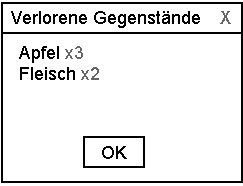
\includegraphics[width=0.4\columnwidth]{figures/wireframes/lost-items.pdf}
    \caption{\label{fig:lostitems}Verlorene Gegenstände}
\end{figure}

Die höchste positive Zustimmung hat die Hypothese erhalten, dass verlorene Gegenstände nach dem Verlust eines Lebens, der spielenden Person, angezeigt werden sollen.
Die Umsetzung dieser Funktionalität kann mithilfe eines zusätzlichen Pop-ups bewerkstelligt werden.
Der Inhalt in \autoref{fig:lostitems} zeigt alle Gegenstände an, welche verloren gegangen sind.
Ebenfalls wird die Menge angegeben.
Das Pop-up kann entweder mit dem OK-Knopf oder dem Kreuz verlassen werden. \\

Aufgrund der hohen Korrelation zwischen der Möglichkeit ein Geschlecht auszuwählen und dem Charakter Accessoires zu geben ist die Idee aufgekommen, dass ein Charakter-Editor sinnvoll wäre.
Dieser beinhaltet zunächst die Auswahl zwischen einigen Geschlechtern.
Dies erscheint allerdings nur bedingt sinnvoll, weil das Geschlecht im finalen Produkt keine Rolle spielen soll.
Ebenfalls ist keine eindeutige Zuordnung zwischen Aussehen und Geschlecht möglich, weil dieses divers ausfallen kann.
Spielende könnten über fehlerhafte oder mangelnde Pronomen verärgert werden\cite{rockpapershotgun-gender}. \\

\begin{figure}[H]
    \centering
    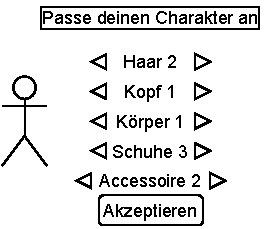
\includegraphics[width=0.5\columnwidth]{figures/wireframes/charselect.pdf}
    \caption{\label{fig:charselect}Charakter-Editor}
\end{figure}

Aus diesem Grund können Spielende über den Charakter-Editor den Charakter selber anpassen und personalisieren.
Ebenfalls sollen Spielende im Spiel nicht mit Pronomen angesprochen werden.
Diese Idee ist in \autoref{fig:charselect} zu sehen.
Die Auswahl an veränderbaren Eigenschaften beschränkt sich zunächst auf die abgebildeten Elemente.
Diese können mithilfe der Pfeile verändert werden.
Die Zahl hinter einem Element bildet die aktuelle Auswahl ab.
Diese kann dann mithilfe des Akzeptieren-Knopfes bestätigt werden. \\

Die Umfrage hat ergeben, dass Personen sich einen Indikator für vergangene Zeit nach einer Aktion wünschen.
Dies zeigt, dass für Spielende an mehreren Stellen nicht klar kommuniziert wurde, wie viel Zeit eine bestimmte Situation in Anspruch nimmt.
Deshalb kann dafür gesorgt werden, dass Hervorhebungen in Dialogen oder Animationen genaue Zeitangaben vermitteln.\\

Das Kampfsystem zu optimieren ist eine der schwierigsten zu bearbeitenden Hypothesen.
Das liegt daran, dass dies eine Kernmechanik ist und Änderungen dazu führen können, dass sich der Kerninhalt des Spiels ändert.
Die Änderung muss dabei zum Gesamtbild des Spiels passen.
Ebenso müssen die Wünsche der beiden Personas befriedigt werden.
Zum einen ist es wichtig, dass mehr Interaktionen möglich sind, zum anderen muss das Spiel auf passive Art und Weise spielbar sein.
Dies steht in einem starken Kontrast zueinander. \\

Aus diesem Grund ist die erste Idee, die Interaktionen nicht nur während des Kampfes, sondern auch vor dem Kampf zu erhöhen.
Sobald ein Kampf stattfindet, soll die spielende Person zunächst eine Phase der Vorbereitung durchlaufen.
Dort können Aktionskarten zu einem Kartendeck zusammengestellt werden.
Die auswählbaren Karten sind abhängig vom Typ des Digimons.
Ebenfalls wird die Mechanik verworfen, Gegenstände im Kampf zu verwenden.
Diese Mechanik wird durch die neuen Aktionskarten ersetzt.
Im Kampf bestimmt die aktuelle Menge von Magie, welche Karte ausgespielt werden kann.
Die Idee ist, dass Karten Angriffe oder Effekte erzwingen können, welche der Partner sonst nur zufällig auswählen kann.
Die Angriffe haben dann jeweils abhängig der Intelligenz des Partners eine prozentuale Chance den Gegner zu treffen.
Schwächere Angriffe haben eine hohe und stärkere Angriffe eine niedrige Chance zu treffen.
Dadurch entsteht eine Relation zwischen Belohnung und Risiko.
Dies soll den spielenden taktische Entscheidungen ermöglichen. \\

Digimon World besitzt das Problem, dass an einigen Stellen im Kampf ein Stunlock vorkommen kann.
Das bedeutet, dass ein Gegner permanent angegriffen wird, ohne reagieren zu können.
Dies passiert primär bei zu hoher Geschwindigkeit, weil der Gegner seinen Angriff immer langsamer ausführt als das eigene Digimon.
Um dieses Problem zu beseitigen, sollen Digimon Angriffe nacheinander ausführen.
Dies gleicht einer rundenbasierten Kampfmechanik. \\

Dieses System wurde mehrfach überarbeitet, weil es viele Probleme beinhaltet.
Das erste Problem ist, dass die klare Trennung zwischen Digimion und der spielenden Person verloren geht.
In dieser Kampfmechanik agiert nur die spielende Person.
Gleichermaßen wird die Persona Elena keine Möglichkeit haben, das Spiel zur Entspannung zu verwenden, weil das Kartensystem eine zu hohe Komplexität besitzt. \\

\begin{figure}[H]
    \centering
    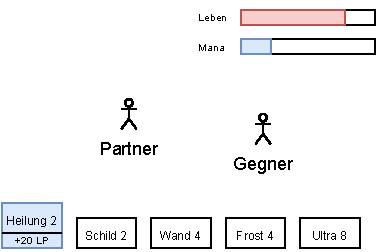
\includegraphics[width=0.8\columnwidth]{figures/wireframes/battle.pdf}
    \caption{\label{fig:battle-wireframe}Kampfsituation}
\end{figure}

Nach mehreren Iterationen der Optimierung ist das gewünschte Ergebnis erreicht.
Dieses ist in \autoref{fig:battle-wireframe} dargestellt.
Für die Erklärung wird anfänglich das Kampfsystem von Digimon World als Basis genommen.
Zunächst wird die maximale Menge an verfügbaren Magiepunkten auf zehn reduziert.
Diese war zuvor variabel. Ebenfalls startet jeder Kampf mit drei Magiepunkten.
Die Idee, Karten im Kampf verwenden zu können, wird zunächst von der vorherigen Iteration übernommen.
Allerdings erzwingen diese keine Angriffe, sondern wirken unterstützende Effekte.
Dadurch kann der Partner alleine agieren und die spielende Person wirkt als Unterstützer.
Dies hat zur Folge, dass weiterhin eine klare Trennung zwischen beiden Charakteren existiert.
Die verfügbaren Aktionskarten unterscheiden sich pro Partner und können vom Typ abhängig sein.
Jeder Partner besitzt fünf verfügbare Aktionskarten.
Die Kosten für diese belaufen sich auf zwei, zwei, vier, vier und acht Magiepunkte.
Je mehr eine Aktionskarte kostet, desto wirkungsvoller ist diese.
Durch jene Verteilung entstehen zwei Vorteile.
Zum einen die Relation zwischen Belohnung und Risko, zum anderen verschiedene Optionen für die taktischen Entscheidungen.
Die Karte für acht Magiepunkte ist sehr mächtig, allerdings muss abgewogen werden, ob der Partner nicht früher auf andere Aktionskarten angewiesen ist.\\

Im Kampf sollen im Vorfeld bereits mehr der in Digimon World vorkommenden Optionen verfügbar sein.
Das bedeutet, dass die Optionen aggressiver, defensiver oder scheuer Spielstil bereits zu Beginn verfügbar sind.
Dadurch wird der Parameter Intelligenz vom Kampf entkoppelt.
Diese Optionen sind nicht in \autoref{fig:battle-wireframe} modelliert.
Das liegt daran, dass die Verhaltensweisen in einem weiteren Schritt in der Zukunft zunächst näher untersucht werden müssen.
Das Spiel rundenbasiert zu entwerfen widersetzt sich der Natur des Spiels.
Aus diesem Grund soll der Stunlock durch einen Rückstoß ersetzt werden.
Ebenfalls wird bei jedem Angriff beiden Gegnern Schaden zugefügt.
Magiepunkte können aufgeladen werden, wenn die spielende Person kurz vor einem Angriff eine entsprechende Taste betätigt.
Falls eine Person kein Interesse an dieser Funktionalität hat, kann dies in den Spieleinstellungen deaktiviert werden.
Aus Sicht von Christian ensteht durch diese neue Kampfmechanik mehr taktisches Vorgehen und mehr Interaktion.
Elena hingegen besitzt weiterhin die Option, dem Partner beim Kämpfen zuzusehen und einen simpleren Spielstil zu wählen.\\

\begin{figure}[H]%
    \centering
    \subfloat[\centering Final Fantasy XIV]{{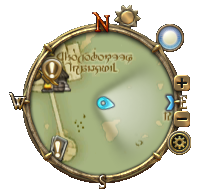
\includegraphics[width=4cm]{figures/screenshots/ff14.png}
                \label{fig:ff14}}}%
    \qquad
    \subfloat[\centering Wireframe]{{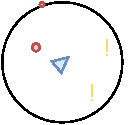
\includegraphics[width=4cm]{figures/wireframes/minimap.pdf} }\label{fig:minimap-wireframe}}%
    \caption{Minimap in Anlehnung an Final Fantasy XIV}%
    \label{fig:minimap}%
\end{figure}

Eine der gänzlich neu hinzugefügten Funktionalitäten ist die Minimap\footnote{Miniaturkarte}.
Diese wurde sich vermehrt von den befragten Personen gewünscht, weil die Spielwelt alleine nicht übersichtlich genug ist.
Aus der Analyse ist hervorgegangen, dass die Existenz und zusätzliche Informationen auf der Minimap mit einer Aufgabenliste korreliert.
Die Aufgabenliste wird später in diesem Abschnitt erwähnt.
Eine mögliche Interpretation dieser Korrelation ist in \autoref{fig:minimap} zu sehen.
Dabei lehnt sich die entwickelte Minimap an die im Spiel Final Fantasy XIV vorkommende Minimap an.
Im Wireframe markieren gelbe Ausrufezeichen offene Aufgaben und rote Punkte Gegner.
Wenn ein Symbol aus dem sichtbaren Bereich der Minimap verschwindet, wird dieses Symbol verkleinert am Rande der Minimap dargestellt.
Das sorgt dafür, dass die spielende Person die ungefähre Position eines Ziels ermitteln kann.
Die spielende Person wird durch ein blaues Symbol dargestellt.
Die Position ist innerhalb der Minimap immer zentriert und die Ausrichtung gibt die aktuelle Rotation in der Spielwelt an.

\begin{figure}[H]
    \centering
    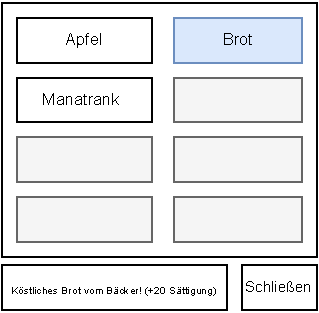
\includegraphics[width=0.5\columnwidth]{figures/wireframes/inventory.pdf}
    \caption{\label{fig:inventory}Inventar}
\end{figure}

Zusätzliche Informationen im Inventar korrelieren mit zusätzlichen Fortschrittsbalken für Sättigung und Toilettenbedarf.
Die vorgenommene Änderung beläuft sich nur auf Textinhalte im Inventar.
\autoref{fig:inventory} zeigt beispielhaft den ausgewählten Gegenstand Brot.
Die Beschreibung gibt an, welche Attribute des Partners sich bei einer Verwendung des Gegenstands verändern.
Bezüglich des Inventars wurde eine weitere Entscheidung getroffen.
In Digimon World wird das Inventar für viele Zwecke verwendet.
Dementsprechend erhöht sich die Häufigkeit, wie oft die spielende Person dieses Menü betrachtet.
Wenn ein Digimon Hunger hat, muss es mit Nahrungsmitteln gefüttert werden.
Manchmal kommt es vor, dass eine Nahrungsration nicht ausreicht.
Das Problem ist allerdings, dass sich das Inventar nach jeder Anwendung einer Nahrungsration schließt.
Dieses Problem soll künftig vermieden werden.
Ebenfalls existiert für das Inventar kein Zwischenmenü.
Dies verringert die Benutzungstiefe.
Das Inventar wird im neuen Spiel dann standardmäßig mit der Taste \texttt{I}, für Inventar oder Inventory, geöffnet.
Das Inventar besitzt begrenzte Plätze und es ist zunächst nicht geplant, dass diese erweitert werden können.
Die Begrenzung soll dafür sorgen, dass Spielende sich bewusst dazu entscheiden, welche Vorräte sie bei der Erkundung benötigen.\\

\begin{figure}[H]
    \centering
    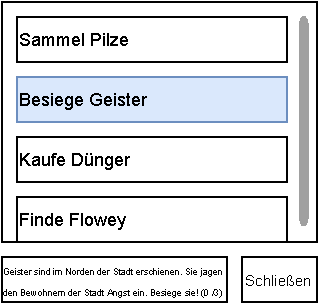
\includegraphics[width=0.5\columnwidth]{figures/wireframes/journal.pdf}
    \caption{\label{fig:journal}Aufgabenliste}
\end{figure}

\autoref{fig:journal} zeigt ein Wireframe für die Aufgabenliste.
Die Aufgabenliste ist ähnlich zum Inventar aufgebaut.
Jedoch ist die Anzahl der annehmbaren Aufgaben nicht begrenzt.
Die Spielenden sollen frei entscheiden, welchen Aufgaben sie sich zuerst widmen.
Bei der Auswahl einer Quest wird diese farblich hervorgehoben und eine Beschreibung erklärt detailliert, was getan werden muss, um die Aufgabe zu erfüllen.
Ebenfalls ist es wie beim Inventar möglich, das Journal mit einer Taste zu öffnen.
Die hierfür gewählte Taste ist \texttt{J}.
Diese Taste ist ebenfalls eine typische Abkürzung in Videospielen und steht für Journal.
Geschlossen werden können beide Menüs mithilfe des Schließen-Knopfes, der Betätigung der entsprechenden Taste (\texttt{I}/\texttt{J}) oder der \texttt{ESC}-Taste.\\

Eine andere Funktionalität, welche sich oft gewünscht wurde, sind weitere visuelle Hinweise, wie beispielweise Knöpfe im \ac{HUD}.
Diese sollen angezeigt werden, wenn der Videospielcharakter mit einem Objekt oder einem \ac{NPC} interagieren kann.
Die Idee ist in diesem Fall, dass der entsprechende Knopf über dem Objekt erscheint, wenn sich der Spieler im entsprechendem Radius befindet.\\

\begin{figure}[H]%
    \centering
    \subfloat[\centering Uhr in Digimon World]{{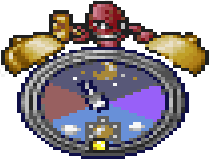
\includegraphics[width=4cm]{figures/screenshots/clock.png}
                \label{fig:clock}}}%
    \qquad
    \subfloat[\centering Fortschrittsbalken]{{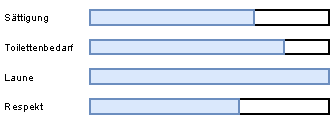
\includegraphics[width=7cm]{figures/wireframes/progressbars.pdf} }\label{fig:progressbars}}%
    \caption{Uhr und Fortschrittsbalken}%
    \label{fig:clock-progress}%
\end{figure}

Die Uhr in Digimon World, welche in \autoref{fig:clock} dargestellt ist, konnte zunächst von den interviewten Personen nicht korrekt gedeutet werden.
Dies brachte die Hypothese auf, dass diese durch eine Uhr mit zwei Zeigern ersetzt werden sollte.
Die Mehrheit der Personen in der Umfrage stimmten dieser Aussage zu.
Das bedeutet, dass in der Implementierung eine Uhr mit zwei Zeigern nötig ist. \\

Aufgrund einer ungünstigen Formulierung in der Umfrage stellte sich heraus, dass Personen kein Interesse daran haben, einen Fortschrittsbalken, welcher zwei Mal voll werden muss, in einen Fortschrittsbalken zu ändern, welcher nur einmalig gefüllt werden muss bis der Maximalwert erreicht ist.
Teilnehmende Personen der Umfrage haben die Aussage, Glück und Disziplin nicht zu spalten, so verstanden, dass Glück und Disziplin ein neuer Wert Glück-Disziplin ist.
Nach einer weiteren Nachfrage stellte sich heraus, dass einige teilnehmende Personen ansonsten zugestimmt hätten.
Aus diesem Grund werden die Fortschrittsbalken so angepasst, dass diese nur ein Mal voll werden können.
Ebenfalls werden weitere Informationen wie Sättigung und Toilettenbedarf hinzugefügt.
Diese sind in \autoref{fig:progressbars} zu sehen.
Zusätzlich werden keine Symbole verwendet, sondern Texte, welche den Inhalt der Fortschrittsbalken beschreiben.
Dies soll Missverständnisse vermeiden.\\

Die Hyptothese, ein Tutorial hinzuzufügen, wird in dieser Arbeit zunächst vernachlässigt.
Das liegt daran, dass diese eine niedrige Bewertung im Ranking besitzt.
Viel wichtiger ist jedoch die Tatsache, dass für die Implementierung zunächst das Kampfsystem und technische Funktionalitäten im Fokus stehen.
Die Erkenntnis, dass das Tutorial im Spiel vorhanden sein muss und damit einen Einstieg im Spiel bietet, ist jedoch deutlich.
Das Tutorial ist nach Implementierung der Kernfunktionalitäten in Form einer spielerischen Anleitung geplant.
Das bedeutet, dass Spieler mithilfe von Aufgaben Menüs, Kampfmechaniken oder die vorhin genannten Funktionalitäten erkunden können.
Texttutorials wurden in Erwägung gezogen, allerdings widersprechen diese dem Persona von Christian.
Dieser möchte Spielinhalte durch Handeln erlernen und keine langen Erklärungstexte lesen.
